\documentclass[a4paper,10pt,twocolumn,uplatex]{jsarticle}
\usepackage{style/nislab,style/resume}
\usepackage[dvipdfmx]{graphicx}
\usepackage{amsmath, amssymb}
\usepackage{bm}

%---------------------------------------------------------------------
% レジュメ種別・日付設定
%---------------------------------------------------------------------
\type{3}
\year{2026}
\month{5}
\date{11}

%---------------------------------------------------------------------
% ページ番号設定
%---------------------------------------------------------------------
\setcounter{page}{9}

\begin{document}

%---------------------------------------------------------------------
% タイトル作成部分
%---------------------------------------------------------------------
\maketitle{協調認識のための交通流予測に基づく
\\帯域適応型V2Xハイブリッド経路制御方式の検討}
{Bandwidth-Adaptive V2X Hybrid Routing Control
\\Based on Traffic Flow Prediction for Cooperative Perception}
{古米 遼成}
{Ryosei Furumai}

%---------------------------------------------------------------------
\section{はじめに}
近年，自動運転の安全性向上を目的として，V2X通信を用いて死角の物標情報を共有する協調認知サービス（CPS）の研究が進んでいる．総務省の自動運転・ITSの通信インフラに関する取組においても，5.9GHz帯のV2X通信とV2N（セルラー網）通信の相互補完的な活用が自動運転の社会実装に向けた重要なインフラ基盤として位置づけられている~\cite{digital_lifeline}．

しかし，高車両密度環境下では，各車両が送信する協調認識メッセージ（CPM）の増大により通信帯域が逼迫し，パケット衝突による高重要度情報の欠落が課題となっている．この課題の解決策として帯域逼迫が発生してから対処する反応型制御があるが，これは急激な変動に対して制御が間に合わず，通信品質の劣化を招く恐れがある．さらに，情報を一律に削除することは，ネットワーク全体の協調認識の精度を低下させる要因ともなり得る．

そこで本研究では，高車両密度環境下における通信信頼性の確保と周辺物標情報の認識率向上を目的とし，路側機（RSU）による交通流観測に基づいた通信帯域適応型V2V/V2Nハイブリッド経路制御を提案する．具体的には，RSUが予測したチャネル混雑度（CBR）に基づき，通信環境を通常・警戒・逼迫の3段階に定義し，情報の重要度に応じて送信経路に選択する．低重要度情報をV2Nへ適応的にオフロードすることでV2V帯域の逼迫を未然に防ぎ，高重要度情報のためのリソースを確保する．帯域逼迫時にはV2Vに加えV2Nへ二重送信することで，高重要度情報の到達信頼性を最大化する．

%---------------------------------------------------------------------
\section{関連研究}
\subsection{山崎らによる冗長性緩和手法}
山崎らは，欧州規格（ETSI）が提唱する3つの冗長性緩和ルール（Frequency・Dynamics・ Distance）を統合し，物標ごとの情報の冗長度を定量評価する統合スコアRを提案した~\cite{山崎2023}．この手法は，自車周囲のCBRの現在値をリアルタイムに監視し，混雑が激しいほどスコアの高い車両情報を優先的に削除することでCPMのサイズを縮小するものである．また，通信機能を持たない歩行者の安全性を確保するため，歩行者情報を極力削除せず，車両情報を優先的に削除する方式を採用している．しかし，この手法はCBRの現在値に基づき混雑が起きてから対処する反応型制御であり，車両密度が急増した際に制御が間に合わない課題がある．

\subsection{Aslamらによる通信路の静的割り当て}
Aslam らは，メッセージの要求遅延や空間的な有効範囲に基づき，V2Vと V2Nを系統的に使い分ける手法を提案した~\cite{Aslam2025}．具体的には，低遅延かつ局所的な共有が求められるCPM等をV2Vに割り当てる一方，広域通知を目的とする地図情報のMAPEM（MAP Extended Message）や，急ブレーキ等の突発的な危険イベントを知らせるDENM（Decentralized Environmental Notification Message）をV2Nへと固定的に割り当てている．しかし，この手法ではV2V帯域が極端に逼迫した際にも特定のメッセージをV2Vに流し続けてパケット衝突を招くなど，状況に応じた柔軟な経路選択ができない課題がある．

%---------------------------------------------------------------------
\section{提案手法}
\subsection{提案手法の概要}
本手法では，RSUによる混雑予見に基づき，情報の重要度（High/Low）に応じて送信経路を選択する．本研究ではDENM等の緊急シナリオは対象外とし，通常メッセージであるCPMの中で，周辺車両との物標情報の重複度（冗長度）や情報の新鮮度（AoI: Age of Information）に基づき，パケットを動的にHigh（高重要）またはLow（低重要）に分類して扱う．V2V帯域の逼迫を未然に防ぐため，予測混雑度 $CBR_{est}$ に応じて通信状態を「通常」「警戒」「逼迫」の3段階に分類する．

\subsection{パッシブリスニングによる負荷観測と混雑予見}
上流の$\mathrm{RSU}_i$は，周辺車両が送信するCPMを受動的に傍受するパッシブリスニングを行う．物理層での誤り検出等により正しく受信されたパケットのみを集計することで，追加のV2V帯域を消費せずに車両密度や速度を算出する．取得された統計情報は，有線ネットワークを介して下流の$\mathrm{RSU}_{i+1}$ へ伝達される．

下流のRSUでは，速度0において無限に発散する問題を回避し，交通流の物理的連続性を表現するため，流体の連続の式に基づく動的時間発展型のCBR予測式を導入する．予測混雑度 $CBR_{est}$ は次式で定義される．
\begin{equation}
CBR_{est} = CBR_{local} + \Delta CBR
\end{equation}
\begin{equation}
\Delta CBR = \frac{(q_{in} - q_{out}) \cdot \Delta t \cdot \lambda \cdot S_{avg}}{R}
\end{equation}
ここで，$CBR_{local}$ は自区間の現在の混雑度，$q_{in}$ は上流からの流入交通量（上流密度 $\times$ 上流速度），$q_{out}$ は自区間から下流への流出交通量（自区間密度 $\times$ 自区間速度）を示す．また，$\Delta t$ は先読み時間，$\lambda$ はメッセージ発生頻度，$S_{avg}$ は平均パケットサイズ [bit]，$R$ はチャネル伝送速度 [bps] である．本式により，分母に速度単体を含まないため車両停止時（速度0）の計算破綻を防ぎつつ，車両の流入に伴う物理的な帯域消費を先回りして正確に推定することが可能となる．

\subsection{混雑状態の定義と適応型経路制御}
本手法では，オフロード開始閾値 $CBR_{start}$ および逼迫閾値 $CBR_{max}$ を用い，表~\ref{tab:data_type}に示す3状態を定義する．各車両は情報の重要度に基づき，最適な経路を選択する．
警戒状態において適用される低重要度情報の V2V 送信確率 $p$ は次式で定義される．
\begin{equation}
p = \max\left( p_{min}, 1 - \alpha \cdot \frac{CBR_{est} - CBR_{start}}{1 - CBR_{start}} \right)
\end{equation}
ここで，$\alpha$ はV2Vでの送信確率を下げるスピードを決める感度係数，$p_{min}$ は最小送信確率である．

\begin{enumerate}
    \item \textbf{通常状態 ($CBR_{est} < CBR_{start}$)}\\
 V2V帯域に十分な空きがあるため，情報の重要度に関わらず全パケットを低遅延なV2Vで送信する．
    \item \textbf{警戒状態 ($CBR_{start} \le CBR_{est} < CBR_{max}$)}\\
 V2Vの効率低下を予見し，低重要度情報のV2V送信確率 $p$ を減少させる．これにより，一部をV2Nへオフロードし，V2V帯域に高重要度情報のための帯域の空きを作り出す．高重要度情報は引き続きV2Vで送信し，低遅延性を維持する．
    \item \textbf{逼迫状態 ($CBR_{est} \ge CBR_{max}$)}\\
 パケット衝突リスクが極めて高い状態であり，制御を強化する．
 \begin{itemize}
    \item \textbf{低重要度情報：} 最小送信確率 $p_{min}$ に基づき，大部分をV2NへオフロードすることでV2Vチャネルの破綻を抑制する．
    \item \textbf{高重要度情報：} V2VとV2Nの二重送信を行う．V2V送信に加えてV2N送信で補完することで，高重要度情報の到達信頼性を最大化する．
\end{itemize}
\end{enumerate}

\begin{figure}[t]
  \centering
  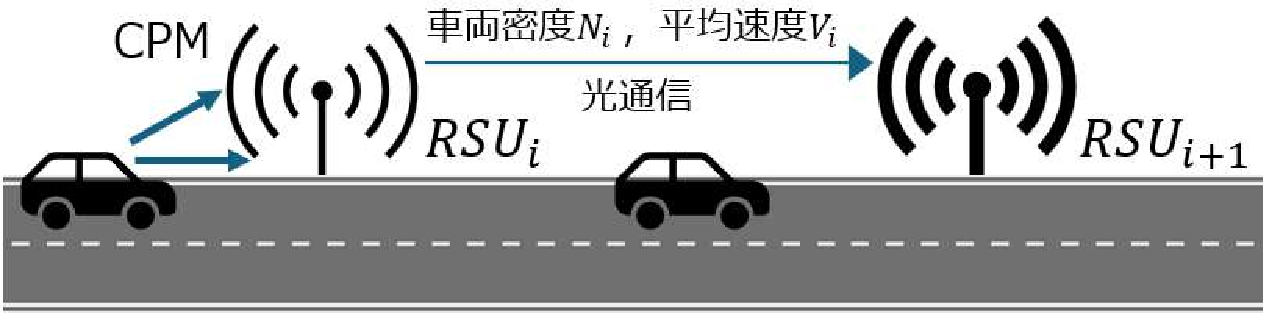
\includegraphics[width=\linewidth]{img/fig1.pdf}
  \caption{RSU連携による混雑予見}
  \label{fig:RSU連携による混雑予見}
\end{figure}
\begin{table}[t]
  \caption{メッセージの送信経路}
  \label{tab:data_type}
  \centering
  \renewcommand{\arraystretch}{1.2} % 行間を少し広げる
  \setlength{\tabcolsep}{10pt}      % 列の余白を調整
  \begin{tabular}{ccc}
    \hline
    V2V帯域状態   & 低重要度情報 & 高重要度情報 \\
    \hline \hline
    通常     & V2V & V2V \\
    警戒 & V2V($p$)$/$V2N($1-p$) & V2V \\
    逼迫 & V2V($p$)$/$V2N($1-p$) & V2V＆V2N \\
    \hline
  \end{tabular}
\end{table}

%---------------------------------------------------------------------
\section{評価方法}
\subsection{評価環境とシナリオ}
VaN3Twinを用い，高速道路（直線道路、2km区間）を想定したシミュレーションを行う．評価車両密度は10台/km（低密度）から250台/km（最高負荷・渋滞発生時）まで動的に変化させる．また，SUMO連携におけるモビリティ計算負荷の増大を防ぎつつ，通信帯域の極限の混雑環境を再現するため，先行研究（山崎氏の修論手法）に準拠したバックグラウンドトラフィックを導入する．具体的には，高頻度（20ms周期 / 50Hz）かつ大容量（1500 bytes）のユニキャスト通信を常時垂れ流す固定のダミー干渉ノードを複数台フィールド内に配置し，意図的にパケット衝突を誘発する最悪条件（Worst-case scenario）を構築して以下の3手法を比較する．
\begin{enumerate}
    \item \textbf{既存手法（RMR）}: 現在のCBRに基づく反応型冗長性緩和手法．
    \item \textbf{適応型冗長性緩和手法}: 予測CBRに基づき RMRを用いて情報の冗長性を緩和する．V2Nへのオフロードは行わない．
    \item \textbf{提案手法}: 適応型冗長性緩和に加え，通信帯域適応型V2V/V2Nハイブリッド経路制御（オフロードおよび二重送信）を統合した手法．
\end{enumerate}

\subsection{評価指標}
\begin{itemize}
    \item \textbf{高重要度情報の到達率（PDR）}: `High` クラスに動的分類された高重要度CPMパケットの到達成功率．
    \item \textbf{周辺物標認識率（ORR）}: 全物標数に対し，V2VまたはV2N経由で正常に情報を受信し，存在を把握できている物標の割合．物標の重複認識や死角による見落としを模擬し，情報の鮮度（AoI）が閾値を超えたものは認識失敗とみなす．
    \item \textbf{冗長性レベルおよび有用性 ($RL, RV$)}: Deloozらが提案する指標を用い，情報の重複度，およびV2NによるV2Vの欠落補完に関する有用性を定量化する~\cite{delooz}．
\end{itemize}

%---------------------------------------------------------------------
%---------------------------------------------------------------------
\section{まとめ}
近年，自動運転の安全性向上のためV2X通信の重要性が高まっているが，高密度環境下ではV2V帯域の逼迫による通信信頼性の低下が大きな課題となっている．本研究では，従来の反応型制御の限界を打破するため，RSUによる混雑予見に基づきV2N帯域を相補的に活用する通信帯域適応型V2V/V2Nハイブリッド経路制御を提案した．

%---------------------------------------------------------------------
\footnotesize{
 \begin{thebibliography}{99}
  \bibitem{digital_lifeline} 総務省, 「自動運転時代の“次世代のITS通信”研究会（第二期） 中間取りまとめ」, 2024年9月.
  \bibitem{山崎2023} 山崎 慎也, 「車両の走行環境を考慮した協調認識メッセージにおける冗長性緩和手法」, 同志社大学 卒業論文, 2023.
  \bibitem{Aslam2025} S. Aslam, et al., "RSU-assisted V2X message fusion via PC5 and Uu with actor--critic modeling for autonomous driving under intersection scenario," Vehicular Communications, vol. 56, 100972, 2025.
  \bibitem{delooz} Q. Delooz, et al., "Analysis and Evaluation of Information Redundancy Mitigation for V2X Collective Perception," IEEE Access, vol. 10, pp. 47076-47093, 2022.
 \end{thebibliography}
}

\end{document}
